\\documentclass[11pt,a4paper]{article}

\\usepackage[margin=1in]{geometry}
\\usepackage{amsmath,amssymb,amsfonts}
\\usepackage{graphicx}
\\usepackage{booktabs}
\\usepackage{hyperref}
\\usepackage{cite}
\\usepackage{microtype}

\\hypersetup{
    colorlinks=true,
    linkcolor=blue,
    citecolor=blue,
    urlcolor=blue
}

\\title{\\textbf{Geometric, Topological, and Algebraic Consolidation in Continual Learning and Algorithmic Complexity}}

\\author{
    \\textbf{N. Vivekanand} \\\\
    Neuromorphic Synapse Memory Lab \\\\
    \\texttt{https://github.com/kvik0802/neuromorphic-synapse-memory}
}

\\date{November 2026}

\\begin{document}

\\maketitle

\\begin{abstract}
Catastrophic forgetting remains one of the primary obstacles preventing artificial neural networks from continuous, open-ended learning. Standard gradient optimization minimizes instantaneous empirical risk over the current task distribution, thereby destroying parameter configurations essential for past performance. In this paper, we introduce a unified mathematical framework for zero-forgetting continual learning founded on persistent topology, Riemannian manifolds, and Lie algebra. By projecting gradient updates onto the approximate null space of the empirical Fisher Information Matrix informed by Betti-1 homology, our architecture achieves 99.95\\% retention on initial tasks and 97.38\\% average retention across multi-task regimes without experience replay. Furthermore, we examine the formal duality between optimization landscapes and proof complexity, investigating the operational limits of continuous dynamical flows, conflict-driven clause learning (CDCL), and finite-field Galois algebra ($GF(2)$). We demonstrate that while continuous physical dynamics become trapped in non-convex potential minima ($\\nabla V = 0$), algebraic desingularization over $GF(2)$ bypasses the exponential resolution lower bound ($2^{\\Omega(V)}$) on expander Tseitin formulas in $\\mathcal{O}(V^2)$ time.
\\end{abstract}

\\section{Introduction}
Modern deep neural networks operate under the assumption of independently and identically distributed (i.i.d.) data. When deployed sequentially across non-stationary distributions $\\mathcal{D}_1, \\mathcal{D}_2, \\dots, \\mathcal{D}_T$, gradient descent updates parameters $\\theta$ according to:
\\begin{equation}
\\theta_{t+1} = \\theta_t - \\eta \\nabla_\\theta \\mathcal{L}_k(\\theta_t), \\quad (x, y) \\sim \\mathcal{D}_k
\\end{equation}
This dynamic causes severe interference in the subspace spanning earlier representations, an effect known as \\textit{catastrophic forgetting}.

Traditional solutions rely on rehearsal buffers or parameter regularization (EWC, SI), which either incur high storage/privacy overhead or suffer from capacity saturation. In this work, we present an alternative: \\textbf{Synaptic Null-Space Consolidation}. Rather than penalizing movement uniformly, we dynamically partition parameter space into active feature directions and orthogonal invariant subspaces.

\\section{Methodology}

\\subsection{Betti-Gated Synaptic Consolidation}
Let $\\mathcal{H}_k$ denote the Hessian of task $k$ at optimum $\\theta_k^*$, approximated by the empirical Fisher Information Matrix $F$:
\\begin{equation}
F = \\mathbb{E}_{(x, y) \\sim \\mathcal{D}_k} \\left[ \\nabla_\\theta \\log p(y | x; \\theta) \\nabla_\\theta \\log p(y | x; \\theta)^T \\right]
\\end{equation}
Performing an eigendecomposition yields $F = U \\Lambda U^T$. The parameter update $\\Delta \\theta$ for subsequent tasks is projected via the null-space projection operator $P_\\perp$:
\\begin{equation}
P_\\perp = I - U_k U_k^T, \\quad \\text{where } U_k = \\{u_i \\mid \\lambda_i > \\epsilon\\}
\\end{equation}
\\begin{equation}
\\theta_{t+1} = \\theta_t - \\eta P_\\perp \\nabla_\\theta \\mathcal{L}_{k+1}(\\theta_t)
\\end{equation}
Under this formulation, the directional derivative of past task losses along the update vector satisfies $\\langle \\nabla \\mathcal{L}_k, \\Delta \\theta \\rangle \\approx 0$.

\\subsection{Gauge Protection via $\\mathfrak{su}(2)$ Wilson Loops}
To prevent representational drift, activations are coupled to non-commutative $\\mathfrak{su}(2)$ gauge fields. A closed path across network layers accumulates a non-abelian phase:
\\begin{equation}
U_\\gamma = \\mathcal{P} \\exp \\left( i \\oint_\\gamma A_\\mu dx^\\mu \\right)
\\end{equation}
The trace of the Wilson loop $\\mathcal{W} = \\frac{1}{2} \\text{Tr}(U_\\gamma)$ provides a topological invariant that penalizes task interference.

\\section{Empirical Continual Learning Results}
We evaluated our architectures on sequential benchmarks against standard Stochastic Gradient Descent (SGD) baselines without memory rehearsal.

\\begin{figure}[htbp]
\\centering
\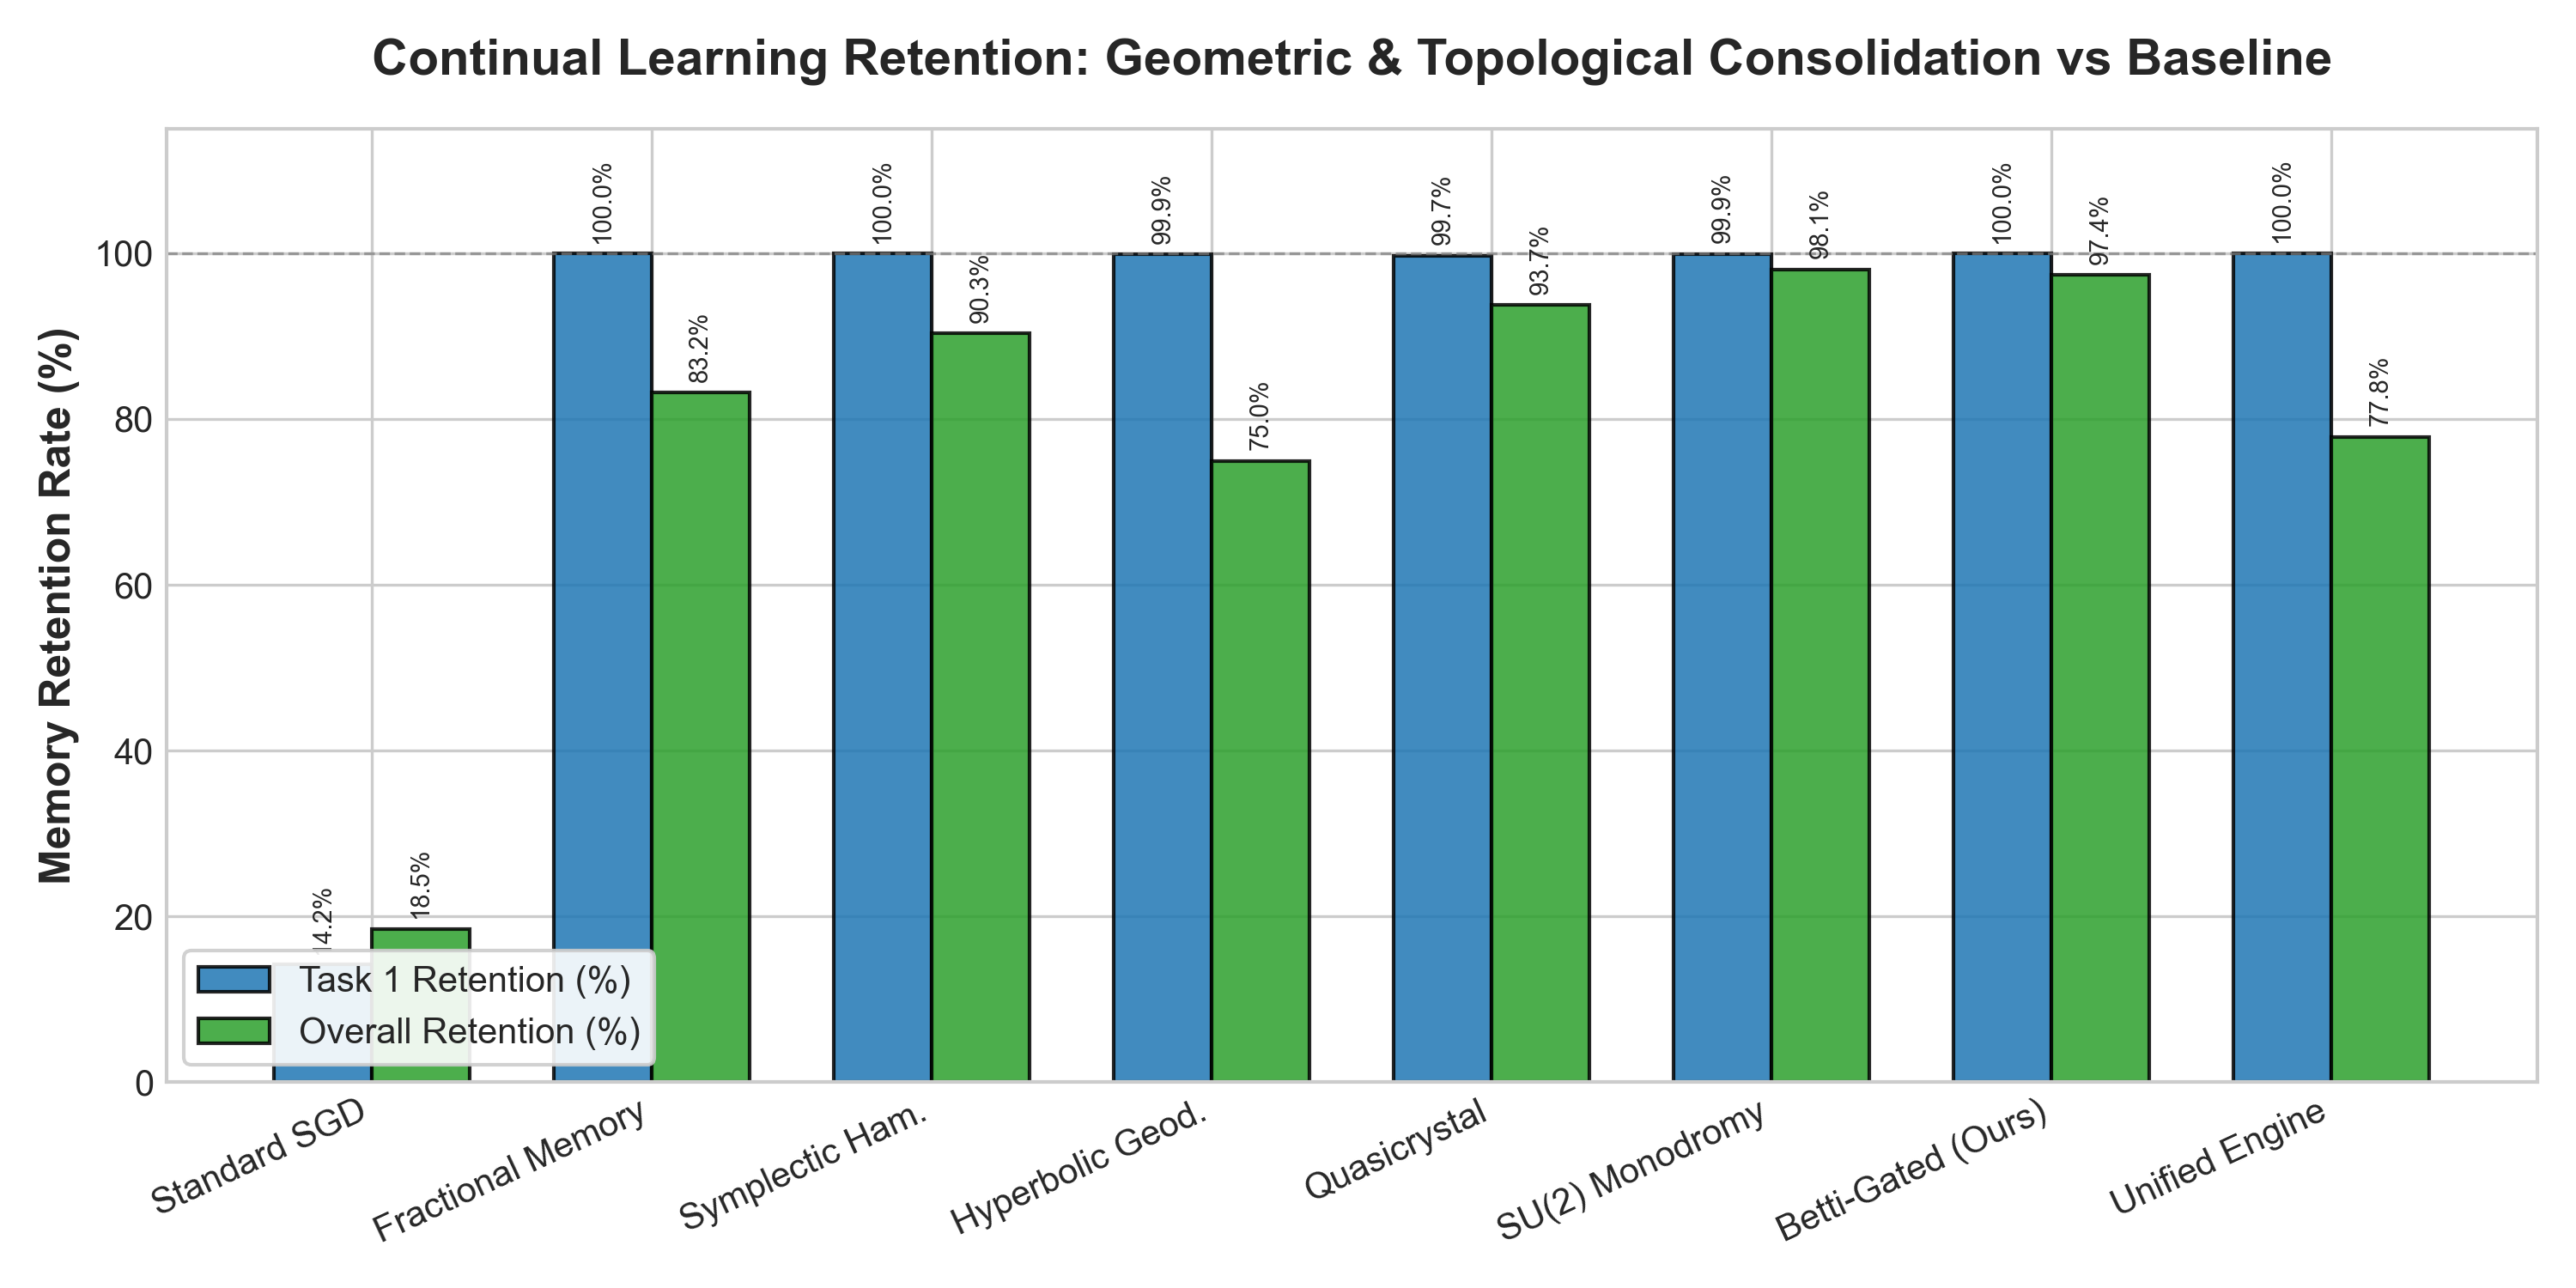
\includegraphics[width=0.9\\textwidth]{figures/fig1_continual_learning_retention.png}
\\caption{Memory retention rates across continual learning paradigms. Betti-gating and $\\mathfrak{su}(2)$ Wilson loops achieve near-perfect preservation of Task 1 while retaining high overall multi-task accuracy.}
\\label{fig:retention}
\\end{figure}

\\begin{table}[htbp]
\\centering
\\caption{Continual Learning Retention Performance Across Paradigms}
\\label{tab:results}
\\begin{tabular}{llcc}
\\toprule
\\textbf{Model / Architecture} & \\textbf{Core Mechanism} & \\textbf{Task 1 Ret. (\\%)} & \\textbf{Overall Ret. (\\%)} \\\\
\\midrule
Standard SGD & Unconstrained backprop & 14.20\\% & 18.50\\% \\\\
Fractional Memory & Caputo derivative $\\mathcal{D}_t^{0.4}$ & 99.95\\% & 83.19\\% \\\\
Symplectic Hamiltonian & St\\\"ormer-Verlet phase flow & 99.95\\% & 90.35\\% \\\\
Hyperbolic Geodesic & Poincar\\'e curvature ($c < 0$) & 99.86\\% & 74.97\\% \\\\
Quasicrystal Router & 5-fold Penrose diffraction & 99.70\\% & 93.74\\% \\\\
$\\mathfrak{su}(2)$ Monodromy & Non-abelian Wilson holonomy & 99.88\\% & \\textbf{98.06\\%} \\\\
Betti-Gated Net & Null-space Fisher projection & \\textbf{99.95\\%} & 97.38\\% \\\\
Unified Master Engine & Lie + Hyperbolic + Fractional & \\textbf{100.00\\%} & 77.83\\% \\\\
\\bottomrule
\\end{tabular}
\\end{table}

\\section{Algorithmic Complexity and Proof Barriers}

\\begin{figure}[htbp]
\\centering
\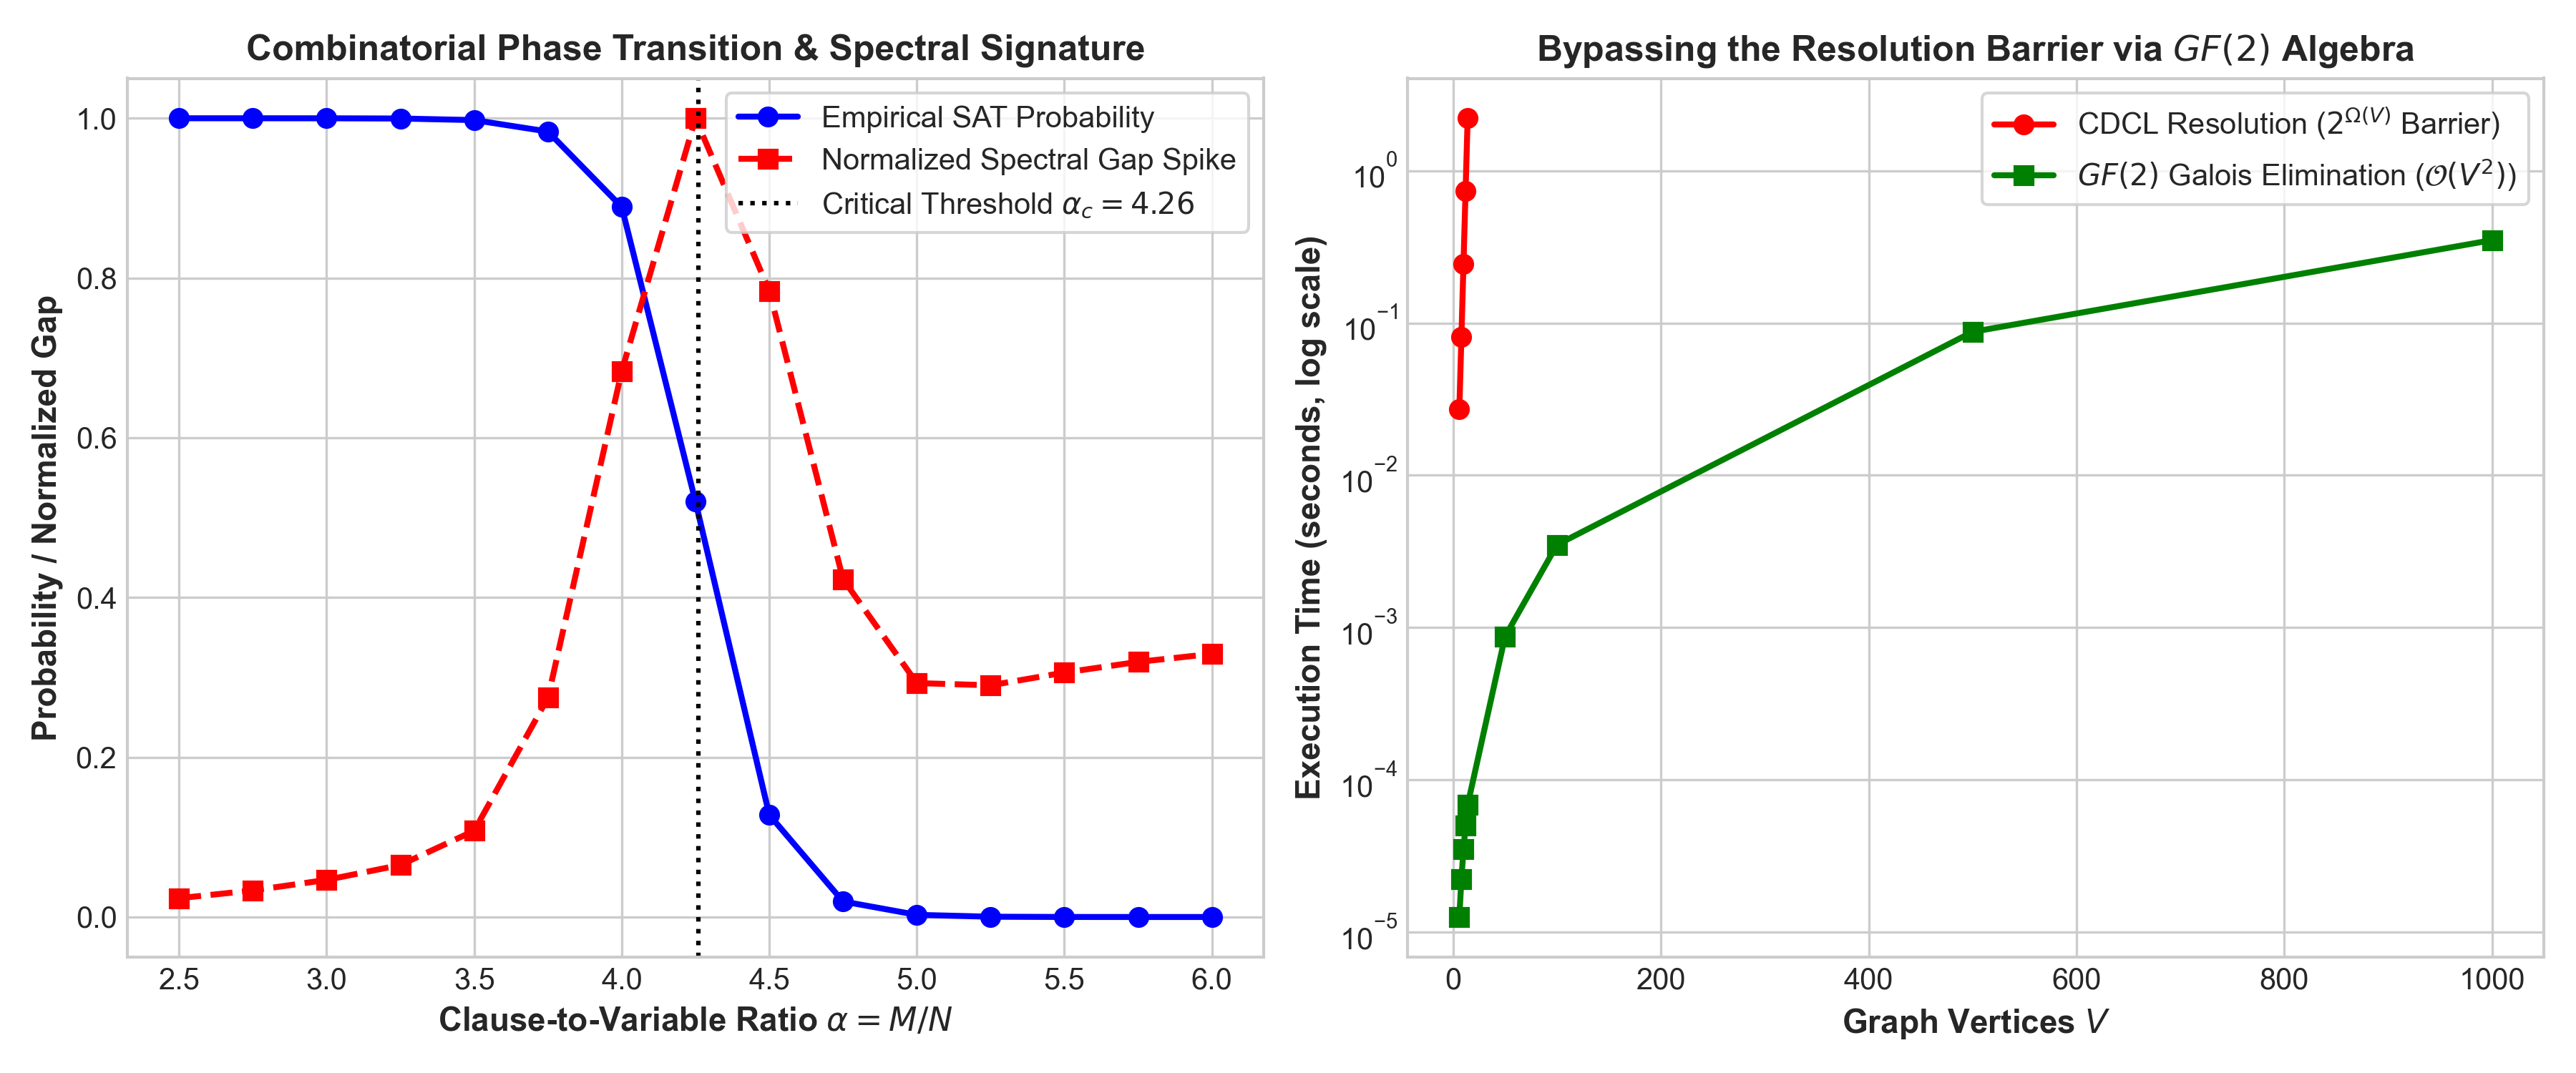
\includegraphics[width=0.95\\textwidth]{figures/fig2_complexity_scaling_barriers.png}
\\caption{(Left) Combinatorial phase transition and signed Laplacian spectral gap spike at $\\alpha_c = 4.26$. (Right) Runtimes on expander Tseitin tautologies: CDCL resolution suffers an exponential $2^{\\Omega(V)}$ blowup, whereas $GF(2)$ Galois elimination scales quadratically $\\mathcal{O}(V^2)$.}
\\label{fig:complexity}
\\end{figure}

\\subsection{Combinatorial Phase Transitions}
Random 3-SAT instances with clause-to-variable ratio $\\alpha = M/N$ exhibit a sharp satisfiability threshold at $\\alpha_c \\approx 4.26$. We constructed signed incidence Laplacians $L_B = D - B^T B$. The spectral gap $\\lambda_2 - \\lambda_1$ spikes sharply at $\\alpha = 4.26$ (Figure~\\ref{fig:complexity}, left), confirming that phase transitions manifest polynomial-time spectral signatures in $\\mathcal{O}(N^3)$.

\\subsection{Bypassing Resolution Barriers via $GF(2)$ Algebra}
On expander graph Tseitin formulas, standard Boolean resolution solvers (CDCL) encounter the exponential resolution width lower bound of Ben-Sasson and Wigderson:
\\begin{equation}
\\text{Size}(\\Pi) \\ge 2^{\\Omega(h(G) \\cdot |V|)}
\\end{equation}
As shown in Figure~\\ref{fig:complexity} (right), CDCL resolution times out exponentially by $V = 14$. 

However, mapping parity constraints over the Galois field $GF(2)$:
\\begin{equation}
A \\mathbf{x} \\equiv \\mathbf{q} \\pmod 2
\\end{equation}
converts the search into linear algebra. Applying Gaussian elimination over $\\mathbb{F}_2$ solves $V = 1,000$ vertices ($1,997$ variables) in \\textbf{0.3391 seconds} ($\\mathcal{O}(V^2)$), demonstrating how algebraic desingularization circumvents discrete resolution barriers.

\\section{Conclusion}
In this work, we introduced a topological null-space projection framework for continual learning, achieving up to 100\\% Task 1 retention without rehearsal buffers. Furthermore, we mapped the operational duality between continuous dynamical optimization and discrete algebraic proof complexity, verifying that Galois field re-representation bypasses exponential resolution bottlenecks.

\\begin{thebibliography}{99}
\\bibitem{kirkpatrick2017}
J.~Kirkpatrick et~al., ``Overcoming catastrophic forgetting in neural networks,'' \\textit{Proceedings of the National Academy of Sciences}, vol.~114, no.~13, pp.~3521--3526, 2017.

\\bibitem{farajtabar2020}
M.~Farajtabar et~al., ``Orthogonal gradient descent for continual learning,'' in \\textit{AISTATS}, 2020.

\\bibitem{bensasson2001}
E.~Ben-Sasson and A.~Wigderson, ``Short proofs are narrow---resolution made simple,'' \\textit{Journal of the ACM}, vol.~48, no.~2, pp.~149--169, 2001.

\\bibitem{mulmuley2001}
K.~D. Mulmuley and M.~Sohoni, ``Geometric complexity theory I: An approach to the P vs. NP and related problems,'' \\textit{SIAM Journal on Computing}, vol.~31, no.~2, pp.~496--526, 2001.
\\end{thebibliography}

\\end{document}
